% ------------------------------------------------------------------------
% -*-TeX-*- -*-Hard-*- Smart Wrapping
% ------------------------------------------------------------------------
%%% Literature Survey --------------------------------------------------

%\addtolength{\topmargin}{-.875in}
%\addtolength{\textheight}{.875in}
%\footskip
%\nonumchapter{Literature Survey}
\chapter{Hybrid Brain-Computer Interface}
\label{chap:hBCI}
\epigraph{Anybody who has been seriously engaged in scientific work of any kind realises that over the entrance to the gates of the temple of science are written the words: Ye must have faith. It is a quality which the scientist cannot dispense with.}{--- \textup{Max Planck}}
%-------------------------------------------------------------------------

\section{Introduction}%Hybrides, Passive, and Neurofeedback
\label{sec:hBCI-intro}

% In rehabilition, one must find a solution which could be adapted to the need and the capacities of each user, because each person is unique.
% people with disability often have residual motor capabilities and want to use it. BCI only system are not robust enough and contradict with the subject's desire to use the working part of their body. A hybrid approach allows the user to combined his residual skills with the possbility of using a BCI to alleviate some boring/repetitive task.
% Claim : We propose a new methodology for disabled people, using an hybrid approach where a physical interface is complemented by a brain computer interface.
% Contribution: Our contribution are threefold : we define a new methodology for design control system for disabled people, we introduce a new learning scheme for BCI and we propose an implementation of  the whole system for two applications in rehabilitation robotics.

Rehabilitation and assistive technologies aim at developing solutions \emph{adapted} to the subjects' disabilities.
A crucial aspect is to take into account the specificities of each person and to propose technical solutions which make use of their residual motor capabilities.
As a simple example, an electric wheelchair will not interest someone who has still some strength in his upper limbs but the same person could be interested by the assistance of an electric motor for driving a manual wheelchair. 
% The aim in rehabilitation and assistive technology is to develop solutions that are adequate to patients' disabilities. 
% Rather than the patients being obliged to adapt to the assistive technologies regardless of their conditions, the approach in rehabilitation is for the assistive technology devices to adapt to the needs of patients, taking into account their disabilities while allowing them to use their residual motor capabilities. 
%Hence in this work, we propose a new methodology for disabled people, using an hybrid approach where a physical interface is complemented by a Brain-Computer Interface (BCI). 

%BCI do not rely on subjects' residual motor capabilities but current system have shown limited performances.
%To overcome these limitations, we design a system that allows the users to use both their brain signals and their residual motor abilities for control tasks.
%Our contribution are threefold : we define a new methodology for a hybrid control system, we introduce a new learning scheme for SSVEP-based BCI and we propose an implementation of  the whole system in two applications of rehabilitation robotics. 

BCI, in their essence, overlook the muscular system. 
They do not rely on subjects' residual motor capabilities. But because of the limited performances of current BCI systems, patients might desire to use their residual motor abilities. 
In this case a system that allows patients to use both their brain signals and their residual motor abilities would be adequate and in-line with rehabilitation principles. 

Hence, in this work, we propose a new methodology for disabled people, using a hybrid approach where a physical interface is complemented by a brain-computer interface. 

The contribution is threefold : we define a new methodology for a shared control system, we introduce a new learning scheme for BCI and we propose an implementation of the whole system in two applications of rehabilitation robotics. 

%We propose a new methodology, where the system integrates a BCI as a complementary communication channel. %that uses user's residual motor abilities. 
The proposed system makes use of user's residual motor abilities and offers BCI as an optional choice: the user chooses when to rely on BCI and could alternate between the muscular- and brain-mediated interface at the appropriate time. % best moment. % leaving to the user the choice 
The hybrid system integrates a 3D touchless interface based on IR-sensors~\citep{martin_fast_2012} that captures hand poses % variation in infrared intensity caused by different hand positions, 
and an SSVEP-based BCI. 
Such an approach combines these two interfaces in a multimodal BCI-motor system that takes advantage of both the user's brain signals and her residual motor ability. %ability to use his 

Regarding the touchless interface, the IR-based interface does not need to be held by the user, thus not requiring any grasping capability. 
It provides a three degrees of freedom controller. 
On the neural side, an SSVEP-based BCI is used and a novel algorithm based on Canonical Correlation Analysis (CCA) is used to classify SSVEP epochs.

%\section{Method and Material}
%\label{sec:hBCI-method}
\section{Proposed Hybrid Interface}

The proposed hybrid approach is illustrated in Figure~\ref{fig:hBCI}.
The user -- a person with motor disabilities -- is given two modalities to control the system. 
The first modality is an input device that takes a signal generated by users' motor action. 
This might be any type of device that is adapted to the subject's disability, allowing her to use her residual motor ability. 
This modality is used for the continuous control of the system. 

\begin{figure}[!ht]
    \centering
    %\pgfimage[interpolate=true,width=0.8\columnwidth]{Figures/hBCI2.pdf}
    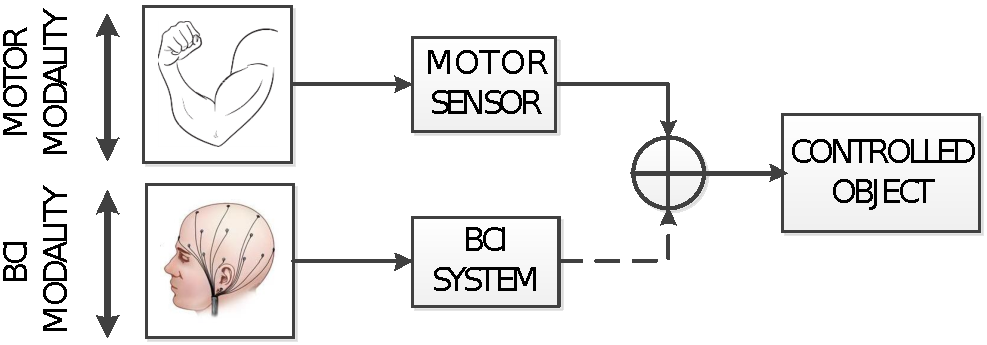
\includegraphics[width=0.8\columnwidth]{Figures/hBCI2.pdf}
    \caption{Hybrid BCI system integration. The motor abilities of the user are the primary controller of the system, using adapted interfaces (here: 3D touchless interface). The brain-computer interface (here: SSVEP) provides a complementary communication channel and is designed to trigger specific actions.}
    \label{fig:hBCI}
\end{figure}

The second modality, which is based on the EEG, is used to provide an additional command, giving alternative control options to the user, or a special command to activate a common and repetitive task.
In this work, the continuous control is achieved by means of a touchless interface and the BCI modality relies on SSVEP. 

\section{Touchless Interface}
\label{sec:touchless-interface}

%- First to equip exoskeleton
%- Then as a general interface that offers many degree of freedom without grasping. It can suitably replace the joistick
There are a number of neurodegenerative diseases that affect large muscles. Some result in loss of strength in the hands and the fingers.
For instance, people with amyotrophic lateral sclerosis may have their hands and fingers weakened and lose their grasping capacity.
Such patients cannot use most of the existing computer input devices such joysticks and mouses that require a certain degree of grasping. 
The \emph{touchless} interface used in this work is designed for such patients. 
It requires no physical contact and no grasping.
The interface embeds five infrared (IR) sensors which could be setup in different spatial positions, according to the user requirements.
Each IR-sensor consist of a pair of IR transmitter-receiver (Tx/Rx). 
The sensors are placed spatially around a user's arm such that a slight hand movement will alter the pattern of reflected IR beams.
The interface is configured to detect six hand positions for six commands namely up, down, left, right, forward, and backward.
To these is added a resting position.
The position is chosen to be intuitive and coherent with the command. They are further tuned to fit user hand movement capacities through a training phase where the subject is asked to perform movements corresponding to the six positions for a number of times.

\begin{figure}[h!]
\centering
\subfigure[]{
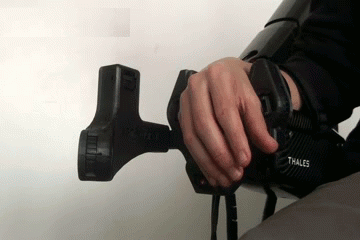
\includegraphics[width=0.3\textwidth]{Figures/left}
\label{fig:ir-left}
}
\subfigure[]{
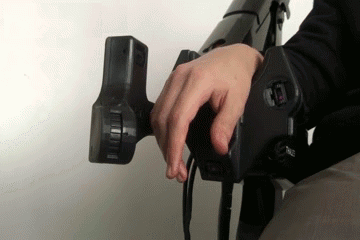
\includegraphics[width=0.3\textwidth]{Figures/right}
\label{fig:ir-right}
}
\subfigure[]{
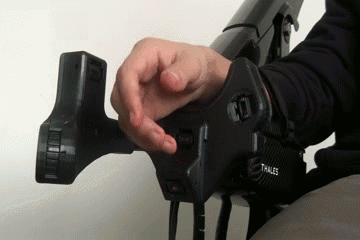
\includegraphics[width=0.3\textwidth]{Figures/up}
\label{fig:ir-up}
}
\subfigure[]{
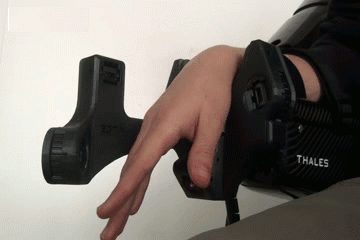
\includegraphics[width=0.3\textwidth]{Figures/down}
\label{fig:ir-down}
}
\subfigure[]{
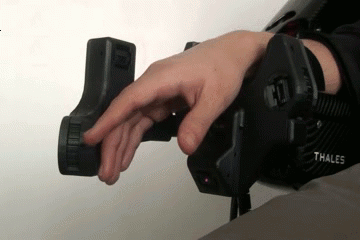
\includegraphics[width=0.3\textwidth]{Figures/front}
\label{fig:ir-front}
}
\subfigure[]{
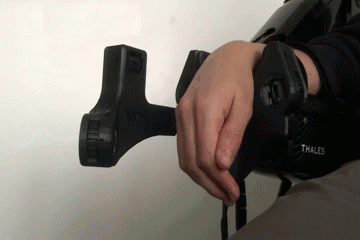
\includegraphics[width=0.3\textwidth]{Figures/rear}
\label{fig:ir-rear}
}
\subfigure[]{
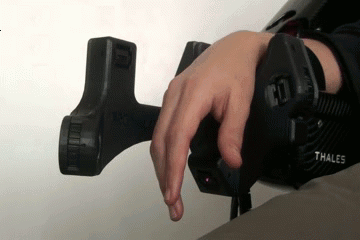
\includegraphics[width=0.3\textwidth]{Figures/rest}
\label{fig:ir-rest}
}
\caption{The 3D touchless interface and a user's hand positions for different commands: (a) left, (b) right, (c) up, (d) down, (e) forward, (f) backward, (g) rest. The IR-sensors are in the black plastic housing on the right side of the hand and around the wrist. Another symmetrical plastic housing has been realised for left-handed users.} 
\label{fig:3D-touchless}
\end{figure}   

The control system relies on an iterative $k$-Nearest Neighbours (kNN) scheme to learn hand poses of each user. 
Firstly, the iterative kNN scheme requires a fast calibration phase to learn the different hand poses, here seven (six for the directions and one for the resting position). 
The outliers and ambiguous examples are excluded from the training examples.
Secondly, the algorithm continuously adapts to the received signal, labelling new examples change the  set of neighbours.
This algorithm is able to track the changes of the user's hand pose, providing an online adaptation to the behavioural modifications induced by tiredness. 
For more details on the algorithm, see\citep{martin_fast_2012}.
The six hand positions recognised by IR-interface is used to control a four degrees-of-freedom robotic arm exoskeleton developed in the \emph{ESTA} project \citep{baklouti_force_2008} to compensate for motor deficiency in the upper limb (Figure~\ref{fig:esta-expe-setup}). 
More generally, it can be used by patients as well as healthy subjects in applications where navigation in a 3D Euclidean space is needed.  

\section{SSVEP-based BCI}
\label{sec:ssvep-bci}

\subsection{Material and EEG Recording}
\label{subsec:material-recording}
The g.Mobilab+ device (shown in Figure \ref{fig:acquisition-system}) is used for recording EEG at 256~Hz on 8 channels.

\begin{figure}[!h]
    \centering
    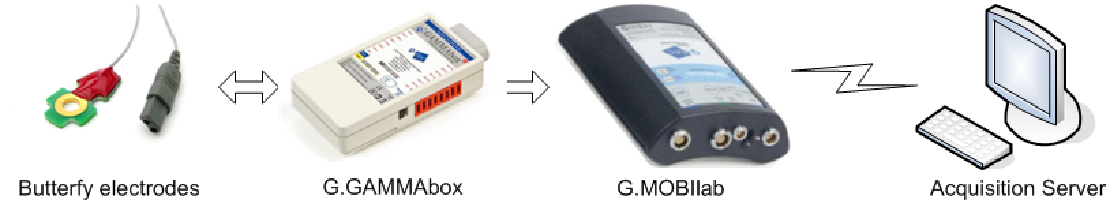
\includegraphics[width=0.8\columnwidth]{Figures/acquisition-system.pdf}
    \caption{\footnotesize{Acquisition material, the EEG is recorded with electrodes, the signal is amplified and sent to a computer running OpenVIBE.}}
    \label{fig:acquisition-system}
\end{figure}

For SSVEP stimulation, flash stimulus technique has been chosen. 
To avoid limitations imposed by refresh rate of computer screens, a microcontroller is set up to  flash stimuli with light-emitting diodes (LED) at frequencies $F =\{13, 17, 21\}$~Hz. %, 17~Hz, and 21~Hz.
The device has been controlled and the LED blinking is precise up to the millisecond.
The eight electrodes are placed according to the 10/20 system on Oz, O1, O2, POz, PO3, PO4, PO7 and PO8. 
The ground was placed on Fz and the reference was located on the right (or left) ear lobe.

In this study, 12 male and female subjects aged between 20 and 32 years participated in the experiment. 
Informed consent was obtained from all subjects, each one has signed a form attesting their consent. 
The subject sits in an electric wheelchair, his right upper limb is resting on the exoskeleton (Figure~\ref{fig:esta-expe-setup}). 
The exoskeleton is functional but is not used in the offline recordings.

\begin{figure}[!t]
    \centering
    %\pgfimage[interpolate=true,width=\linewidth]{Figures/IR_interface}
    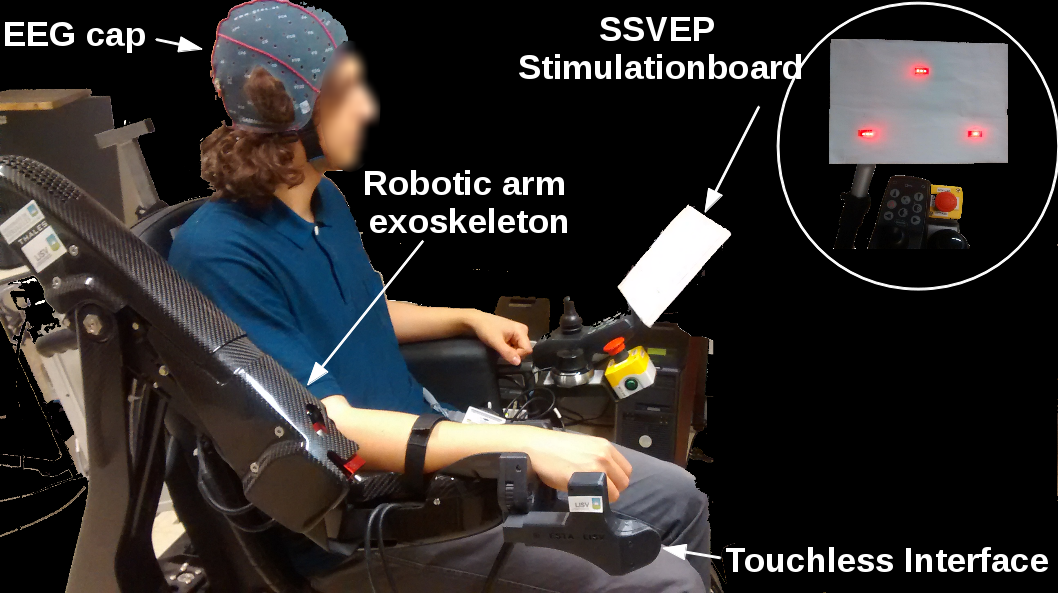
\includegraphics[width=0.8\columnwidth]{Figures/esta-expe}
    \caption{Experimental setting: subject sitting on an electric wheelchair equipped with a robotic arm exoskeleton. During offline recordings, the exoskeleton and the touchless interface are disabled; the subject performs the SSVEP task as prompted by audio cues.}
    \label{fig:esta-expe-setup}
\end{figure}

A panel of size 20x30 cm is attached on the left side of the chair, with three groups of four LEDs blinking at different frequencies. 
Despite the panel being on the left side, users can see it without moving their head. 
The subjects were asked to sit comfortably in the wheelchair and to follow the auditory instructions, they could move and blink freely.
A sequence of trials is proposed to the user. 
A trial begins by an audio cue indicating which LED to focus on, or to focus on a fixation point set at an equal distance from all LEDs for the reject class. 
A trial lasts five seconds and there is a three second pause between each trial. 
The evaluation is conducted during a session consisting of 32 trials, with 8 trials for each frequency and 8 trials for the reject class (or resting class), \textit{i.e.} when the subject is not focusing on any specific blinking LED.

The experiments were conducted at the \emph{Laboratoire d'Ing\'{e}nierie des Syst\`{e}mes de Versailles} (LISV) of the Universit\'{e} de Versailles Saint-Quentin-en-Yvelines, Paris-Saclay. 

\subsection{Signal Processing}

The measured EEG signal is treated with a processing pipeline that offers state-of-the art BCI performance.
EEG epochs of three seconds are gathered every 0.5 second. 
Each epoch is filtered between 12 Hz and 45 Hz to discard irrelevant bands while allowing all stimulation frequencies and their first harmonics. 

A spatial filter is then designed based on CCA method described in Section~\ref{subsubsec:cca}.
Unlike the work of \citep{lin_frequency_2006}, which propose to rely on the correlation coefficient of CCA for processing SSVEP signals, in this work CCA is only applied to determine the spatial filter $w_{\X}$.


%A spatial filter is then designed based on CCA. 
%Let $\X \in \Re^{\dc \times \dt}$ be the obtained EEG trial, where $\dc$ is the number of channels and $\dt$ the number of samples in the trail. 
With the signal being recorded at 256 Hz with eight electrodes, the size of a 3-second EEG trial is $8 \times 768$ ($\X \in \Re^{8 \times 768}$). And let $Y \in \Re^{H \times \dt}$ be a multivariate signal representing the SSVEP stimulation signal.
As described in Section~\ref{subsubsec:cca}, CCA finds the mappings $\w_{\X}, \w_{Y} \in \Re^{8}$ that maximises the correlation between the $\w_{\X}^T \X$, and $\w_{Y}^T Y$.
The signal $\x = \w_{\X}^T \X$ is a linear combination of all the electrodes and is expected to maximise the correlation with a hypothetically perfect neural response, that is the sinusoids of $Y$.
A similar approach can be found in~\citep{spuler_one_2012} but in a different context and using $\x$ to generate exemplars for supervised learning.
After filtering, a multiclass SVM classifier with RBF kernels is used for classification (refer to Section \ref{subsubsec:svm}). 
It is given as input the power spectral densities extracted from the spatially filtered signal $\x$, and output a class $\ci \in \left\lbrace 13 \mathrm{Hz}, 17 \mathrm{Hz}, 21\mathrm{Hz}, resting \right\rbrace$.
The LIBSVM \citep{chang_libsvm:_2011} package is used for SVM implementation.

\section{Applications}

The described approach is validated in two contexts: a Virtual Environment (VE) for the navigation of a helicopter shown in Figure~\ref{fig:online-VE-setup}, and an exoskeleton arm control task shown in Figure~\ref{fig:esta-expe}.
In the VE, the user is asked to reach three waypoints.
Three specific locations are identified in the VE to serve as \emph{shortcuts}. 
In previous works, locations of this nature have been used as a predefined final destination~\citep{lotte_exploring_2010}, while we only use them as shortcuts. 
%They are limited in number to feat the limited number of commands that BCI usually provide. 
After reaching these locations using BCI commands, the user could reach any position using the 3D-touchless interface. 
%is given the option of reaching an infinite number of destinations using the 3D-touchless interface. 

The approach with the exoskeleton arm bears some similitude with the VE navigation task. 
The arm is controlled with the 3D-touchless interface.
Common arm movements performed by the user are predefined (e.g. reaching the mouth or a resting position). 
The BCI shortcut trigger the automatic arm movement to these positions.
 
The hybrid scheme is especially well suited for exoskeleton arm control task: 
%For the robotic arm, this is of essential importance.
as the arm is continuously controlled by the 3D touchless interface, once the user has grabbed an object (e.g. a glass of water), she will no longer be able to move her hand freely to control the touchless interface. 
The BCI command allows to overcome this limitation by activating predefined movements.

\section{Experimental Results}
\label{sec:hBCI-results}
       
This section describes the results obtained with the proposed system.
Out of twelve subjects who participated in the offline EEG recording, only five participated in the online experiment in the virtual environment.
%Five subjects out of participated in the experiments. 
One of the subjects is hemiplegic and the four others are healthy. 
The first section is dedicated to the assessment of the proposed online detection of SSVEP algorithm.
The second section provides the results obtained using the hybrid system for a navigation task in a virtual environment.
The last section explained how the system has been implemented on an embedded system for an exoskeleton arm control task.

\subsection{Validation of Proposed SSVEP Algorithm}
\label{sec:resssvep}

\newcommand{\win}{\ensuremath{t_W}}

Before using the BCI subsystem in online mode, a calibration phase is needed to compute the CCA spatial filter and training the SVM classifier.
During the calibration phase, a sequence of trials is proposed to the user.
%A trial begin by an audio cue indicating which LED to focus on, or to focus on a fixation point set at an equal distance from all LEDs for the reject class.
%A trial last 5 seconds and there is a 3 second pause between each trial.
%The evaluation is conducted during a session consisting of 32 trials, with 8 trials for each frequency $f \in F$ and 8 trials for the reject class, \textit{i.e.} when the subject is not focusing on any specific blinking LED. 
The online classification is done every 0.5 second, using a $\win = 3$~s window of EEG signals. 
An audio feedback indicates the predicted class to the user. %success or failure in the classification. 
%A classification is done every 2 second on the latest EEG sample of 3 seconds.  
%The classification accuracies are given in table~\ref{tab:online_accuracy}.

Figure~\ref{fig:error_rate} shows the online BCI classification performances for each prediction made every 0.5 second, starting at $t=t_0+\win$, that is three seconds after the beginning of the trial $t_0$. 
The y-axis indicates the error rate for each of the five subjects.
The results demonstrate that the proposed algorithm is very robust and provides a very reliable response after $t+2$~s with a small mean error rate for all subjects. 

To further evaluate the algorithm, it is important to consider that the loss function is not uniform. 
If the algorithm detects a reject class instead of a specific class, the consequences are not as bad as a wrong prediction: e.g. detecting 13~Hz instead of 17~Hz, as the user needs only to concentrate half a second on the chosen LED before the system make another prediction.
Thus we propose the following accuracy measure, similar to a precision score.
For each trial, we consider the first class prediction at time $t$: if this is correct the accuracy is increased, if this is false the accuracy is decreased.
If the prediction is the reject class, the accuracy measure is only postponed on the next time segment.
Figure~\ref{fig:accuracy} displays the results of this measure for all subjects.
The accuracy is above 70\% for almost all subjects and it can be seen that the algorithm provides almost immediately the correct answer.
%Table~\ref{tab:online_accuracy} summarizes the maximal accuracy achieved for each subject.

At last, we compare the proposed algorithm with classical SSVEP approaches in Table~\ref{tab:none_ica_cca}, using an offline evaluation  for each subject. 
The baseline is a comparison with a SVM using the PSD of the EEG signal, that is without applying the CCA spatial filter.
A classical methodology is to rely on ICA to extract the main components of the signal and to provide these components to the SVM classifier.
Table~\ref{tab:none_ica_cca} shows that the proposed algorithm yields the best results.

% with a plot of the average classification error rate over a 6.5 seconds trial, computed every 0.5 second for each subject.
% On Figure~\ref{fig:accuracy}, the average accuracy convergence over a 6.5 second trial is plotted for each subject. 
% To evaluate the impact of CCA on the classification, we compare, in table ~\ref{tab:none_ica_cca}, the performance of this technique to the one obtained when no spacial filter is used and the one where ICA is used instead. This was than offline. 

\begin{figure}[!t]
    \centering
    %\pgfimage[interpolate=true,width=0.9\columnwidth]{Figures/error_rate.pdf}
    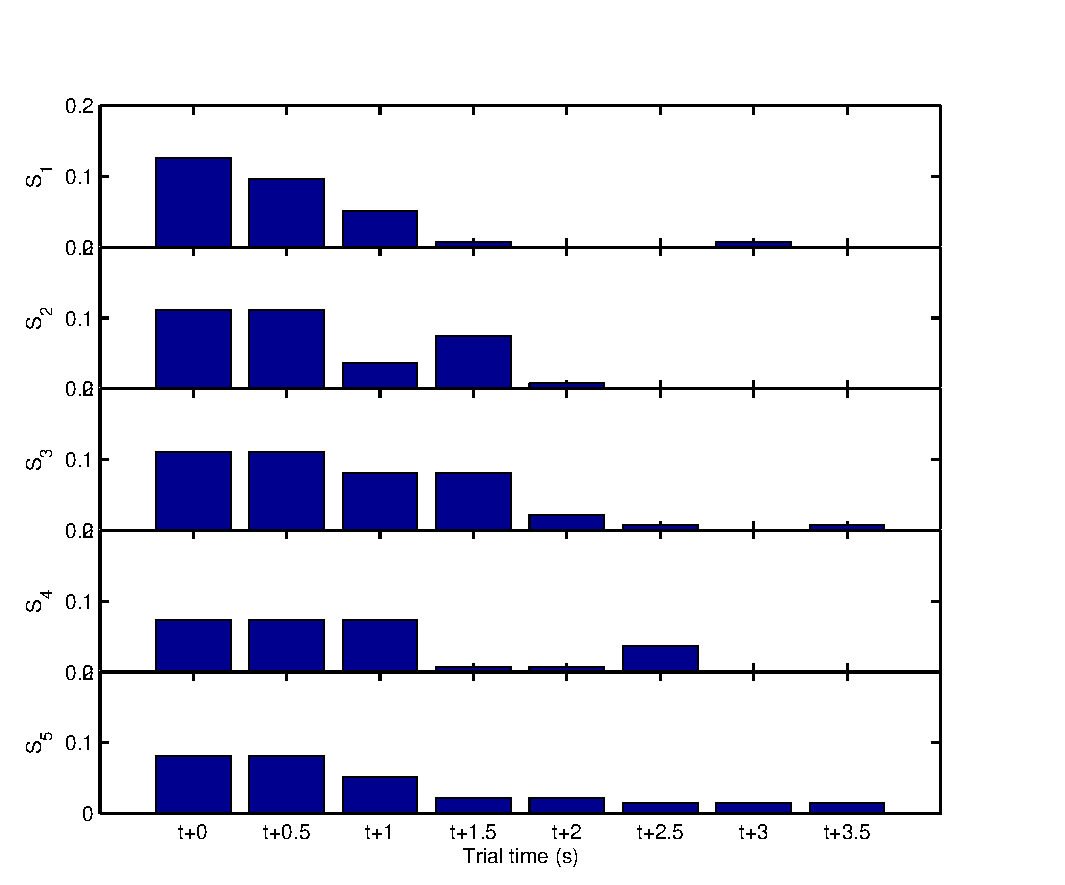
\includegraphics[width=0.8\columnwidth]{Figures/error_rate.pdf}
    \caption{Evaluation of the online performances of the proposed BCI algorithm. The error rates for all five subjects are indicated as a function of time, with $t$+0 indicating the first prediction made (after $\win = 3$~s). The error rates are averaged on all classes.}
    \label{fig:error_rate}
\end{figure}

 \begin{figure}[!t]
    \centering
    %\pgfimage[interpolate=true,width=0.9\columnwidth]{Figures/accuracy.pdf}
    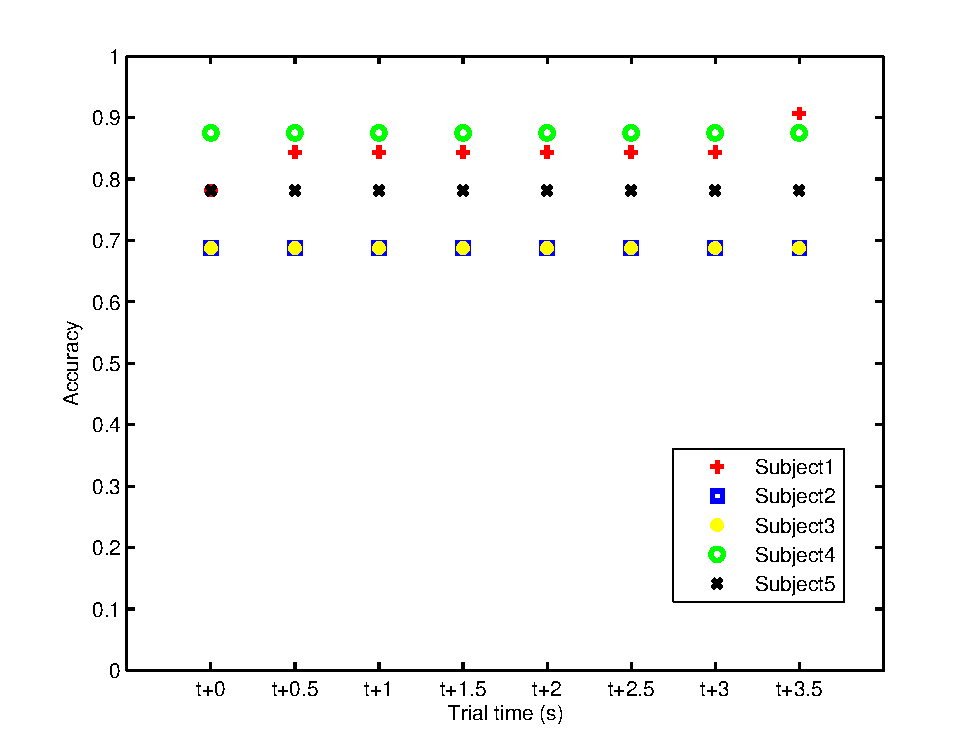
\includegraphics[width=0.8\columnwidth]{Figures/accuracy.pdf}
    \caption{Assessment of the accuracy of classification depending on the time of the prediction. On x-axis, $t$+0 indicates the first prediction made three seconds after the start of a trial. The results are averaged on all trials for each subject. Subject 1 is the only one to present a slight increase of the classification accuracy. For all other subjects, the algorithm proposes a correct answer as the first prediction.}
    \label{fig:accuracy}
\end{figure}

% \begin{table}[!t]
% \centering
% %\ra{1.3}
% \begin{tabular}{@{}lrrrrr@{}}\toprule
% & \multicolumn{1}{c} {Subject1} & \multicolumn{1}{c} {Subject2} & \multicolumn{1}{c} {Subject3} & \multicolumn{1}{c} {Subject4} & \multicolumn{1}{c}{Subject5} \\ \midrule
% Accuracy (\%) & 84.50 & 68.75 & 68.75 & 87.50 & 78.25 \\
% \bottomrule
% \end{tabular}
% \caption{Online accuracy achieved for each subject}
% \label{tab:online_accuracy}
% \end{table}

%\textcolor{red}{table~\ref{tab:online_accuracy} should be updated according to final value of ploss} 


\begin{table}[!t]
\caption{Comparison with other algorithms}
\centering
%\ra{1.3}
\begin{tabular}{@{}lrrrrr@{}}\toprule
& \multicolumn{1}{c} {Subject1} & \multicolumn{1}{c} {Subject2} & \multicolumn{1}{c} {Subject3} & \multicolumn{1}{c} {Subject4} & \multicolumn{1}{c}{Subject5} \\ \midrule
%\cmidrule{2-3} \cmidrule{4-6} \cmidrule{7-9} \cmidrule{10-12}
Baseline& 81.3 & 88.3  & 80.0 & 75.0 & 79.2 \\ \midrule
ICA & \textbf{100} & 88.3  & 91.7 & \textbf{93.3} & 95.0 \\ \midrule
CCA & \textbf{100} & \textbf{100}  & \textbf{97.5} & \textbf{93.3} & \textbf{96.7} \\
\bottomrule
\end{tabular}
\label{tab:none_ica_cca}
\end{table}

\subsection{Experiments in Virtual Environment}
\label{sec:expve}

\begin{figure}[!t]
    \centering
    %\pgfimage[interpolate=true,width=0.8\columnwidth]{Figures/online-expe-setup.jpg}
    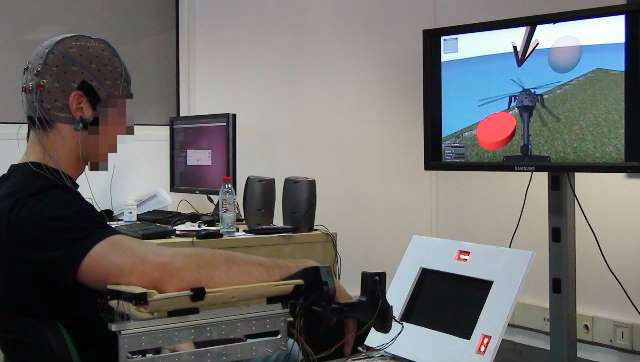
\includegraphics[width=1\columnwidth]{Figures/online-expe-setup.jpg}
    \caption{Experiment in the virtual environment. Here the subject is using the 3D touchless interface with his right hand and the SSVEP LEDs are put in front of him. The screen displays a helicopter in the virtual environment. The subject should pass through all waypoints, materialised by red (or grey) disks on the screen. When the subject triggers a shortcut, the helicopter is automatically moved to a location materialised by the transparent ball.}
    \label{fig:online-VE-setup}
\end{figure}
 
For the navigation task in the virtual environment, the assessment is based on the time spent and the distance travelled during the experiment for four subjects.
%The results in the VE navigation is presented as an evaluation of time spent and trajectory covered to reach the 3 destinations. 
These results are shown in Table~\ref{tab:distime}. 
The time is indicated in seconds and the distance in metric units. 
Each subject has performed three experiments: in the first experimental condition, the subject should rely only on the 3D touchless interface (`None' in Table~\ref{tab:distime}).
In the second one, shortcuts are available and are triggered by the BCI subsystem (BCI-S).
In the last experimental condition, the subject could trigger a shortcut using a keyboard (KB-S).
The fourth subject is hemiplegic and she could not use the keyboard with her spare hand.
Thus, her results do not include the last experimental condition. 

In Table~\ref{tab:distime}, next to the BCI and keyboard shortcut, a percentage indicates the relative improvement compared to the reference experiment (without shortcut).
It could be seen that distance covered is almost equivalent with BCI shortcuts and keyboard shortcuts, which is the expected results as users have activated the shortcut each time it was possible. 
When the shortcuts are activated by the BCI, the task is slower than when using the keyboard. 
This effect is mainly caused because the subject need to focus at least three seconds on a blinking LED before triggering the shortcut. 
%Nonetheless, it could be seen than the subject with hemiplegia could not use the keyboard with his spare hand and thus he could not rely on this alternative to trigger the shortcut.


% , the time spent and the distance covered to reach the destinations when using the 3D touchless interface alone (No short.), are compared with those achieved by using the combination of the touchless interface and shortcuts taken with BCI commands (BCI short.). To evaluate the delay that BCI inserts in the shortcut taking approach, the result are also compared to those achieved when shortcuts are activated by pressing a key on the keyboard (Key short.). The results of 4 subject are shown in table~\ref{tab:distime}. The fourth subject is hemiplegic. His results do not include those of shorcuts activated with the keyboard. Next to BCI short. and Key short. are they respective improvement (increase in performance) factor in percentage compared to the performance of the touchless interface alone.

\begin{table}[!ht]
\centering
\caption{Distance covered and duration of experiments, without shortcuts (None), with BCI-activated shortcuts (BCI-S) and with keyboard-activated shortcuts (KB-S).}
\ra{1.3}
\begin{tabular}{@{}ccrrr@{}}
\cline{1-5}
&  & None & BCI-S (inc. \%). & KB-S (inc. \%). \\ \cline{1-5}
\multicolumn{1}{ c }{\multirow{2}{*}{Subject 1} } &
\multicolumn{1}{ c }{Time} & 108.9 & 68.3 (37.3\%) & 53.56 (50.8\%)      \\ \cline{2-5}
\multicolumn{1}{ c  }{}                        &
\multicolumn{1}{ c }{Distance} & 1367.7 & 538.2 (60.6\%) & 535.0 (60.9\%) \\ \cline{1-5}
\multicolumn{1}{ c }{\multirow{2}{*}{Subject 2} } &
\multicolumn{1}{ c }{Time} & 99.2 & 74.7 (24.7\%) & 50.5 (49.1\%) \\ \cline{2-5}
\multicolumn{1}{ c  }{}                        &
\multicolumn{1}{ c }{Distance} & 1469.4 & 529.1 (64.0\%) & 549.0 (62.6\%) \\ \cline{1-5}
\multicolumn{1}{ c }{\multirow{2}{*}{Subject 3} } &
\multicolumn{1}{ c }{Time} & 105.5 & 63.4 (39.9\%)& 50.4 (52.2\%) \\ \cline{2-5}
\multicolumn{1}{ c  }{}                        &
\multicolumn{1}{ c }{Distance} & 1447.3 & 627.6 (56.6\%) & 542.1 (62.5\%) \\ \cline{1-5}
\multicolumn{1}{ c }{\multirow{2}{*}{Subject 4} } &
\multicolumn{1}{ c }{Time} & 125.6 & 70.4 (43.9\%) & --       \\ \cline{2-5}
\multicolumn{1}{ c  }{(hemiplegic)}                        &
\multicolumn{1}{ c }{Distance} & 1490.8 & 598.9 (59.8\%) & --     \\ \cline{1-5}
\end{tabular}  
\label{tab:distime}
\end{table}
%%\newcommand{\ra}[1]{\renewcommand{\arraystretch}{#1}}
%\begin{table*}\centering
%\ra{1.3}
%\begin{tabular}{@{}rrrcrrcrrcrr@{}}\toprule
%& \multicolumn{2}{c}{Subject1} & \phantom{abc}& \multicolumn{2}{c}{Subject2} & 
%\phantom{abc} & \multicolumn{2}{c}{Subject3} & \phantom{abc} & \multicolumn{2}{c}{Subject4}\\
%\cmidrule{2-3} \cmidrule{4-6} \cmidrule{7-9} \cmidrule{10-12}
%& Time & Distance  && Time & Distance && Time & Distance && Time & Distance\\ \midrule
%Touchless alone & 108.9 & 1367.7 && 99.2 & 1469.4  && 105.5 & 1447.3 && 125.6 & 1490.8 \\
%BCI shortcut & 68.3 & 538.2 && 74.7 & 529.1  && 63.4 & 627.6 && 70.4 & 598.9 \\
%Keyboard shortcut & 53.56 & 535.0 && 50.5 & 549.0  && 50.4 & 542.1 && -- & -- \\
%\bottomrule
%\end{tabular}
%\caption{Distance covered and duration of tasks}
%\label{tab:distime}
%\end{table*}

% The time spent to reach the destinations while using shortucts, BCI or keyboard, is shorter than the time spent when using the touchless interface alone. The difference could be greater in a larger environment. Using a shortcut is definitely a way of fastening and easing the the task. Both BCI and keyboard shortcuts allow users to take predefined optimal paths. They reduce the distance covered by almost equal factors. It is clear when comparing the time of BCI shortcut against the one of keyboard shortcut, that BCI insert a significant delay. Since disabled users, e.g. hemiplegic, cannot reach the keyboard, performances of BCI shortcuts are of great significance.      

\subsection{Application to Exoskeleton Arm Control}
\label{sec:estares}

The proposed system has been applied to the ESTA exoskeleton arm control.
This assistive device is designed to compensate shoulder and elbow deficiencies occurring in degenerative diseases.
The subject controls the exoskeleton arm with the touchless interface and the BCI shortcuts allow to reach predefined positions, such as a resting or a close-to-mouth positions.
In the case of the hemiplegic subject (who cannot use her left arm and hand), the BCI subsystem is the only possibility to control the exoskeleton with an object in hand.
This example illustrates the complementary aspect of the two interfaces, the physical and the brain one.

Figure \ref{fig:esta-expe} illustrates an application of the proposed hybrid interface on the ESTA chair.
The user is seated in an environment where he can perform daily life routine. 
In this case, next to a table where a phone and a glass of water are placed on (to represent objects that are commonly used).
The user can reach to the table, and pick an object of his choice and manoeuvre it around. His arm is supported with the robotic exoskeleton and he is given the touchless interface and the BCI in the hybrid multimodal framework to control it.   
As with in the VR environment, regions of interest can be defined in a daily life environment. 
These regions are the most visited and trajectories leading to them can be optimised and recorded. 
In the current experiment, the table and the user's face (mouth), and the resting positions are defined as regions of interest. 
Their trajectories are optimised, recorded and can be triggered automatically.
In this way, the user can use BCI commands to trigger movement to regions of interest. 
The touchless interface can then be used for it continuous control to reach local positions.
The IR interface can be turned on and off using a BCI command. 
This will allow the user to move his hand even when he does not intend to send a command to the touchless interface.  

\begin{figure}[h!]
\centering
\subfigure[]{
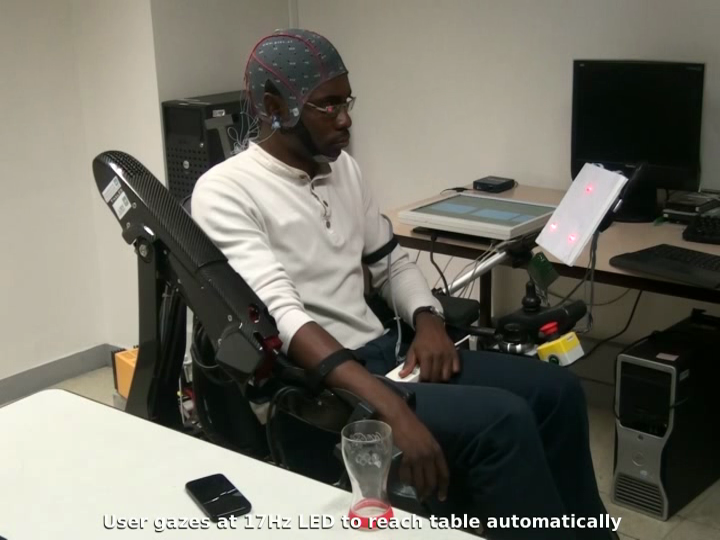
\includegraphics[width=0.45\textwidth]{Figures/esta01}
\label{fig:esta01}
}
\subfigure[]{
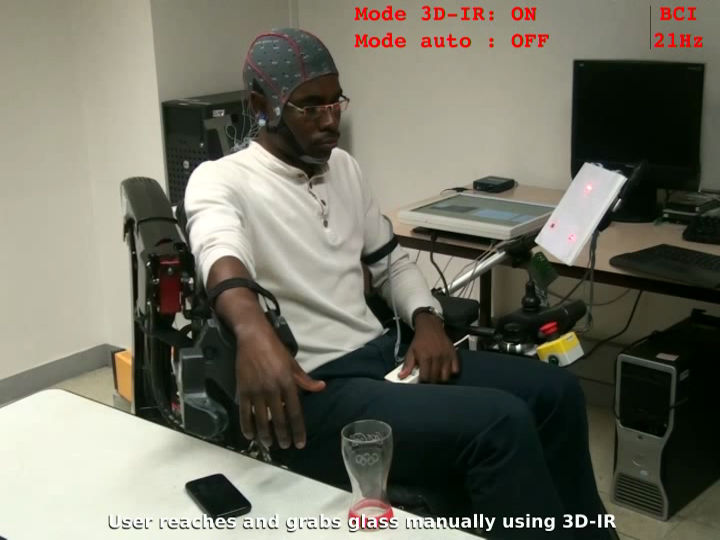
\includegraphics[width=0.45\textwidth]{Figures/esta02}
\label{fig:esta02}
}
\subfigure[]{
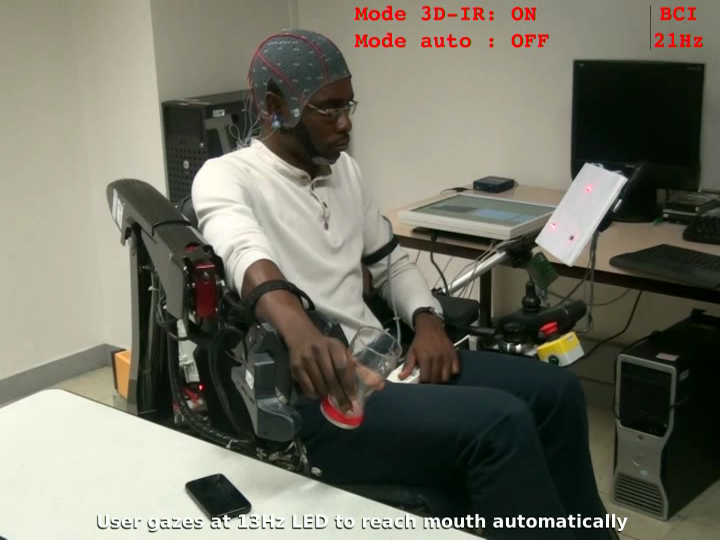
\includegraphics[width=0.45\textwidth]{Figures/esta03}
\label{fig:esta03}
}
\subfigure[]{
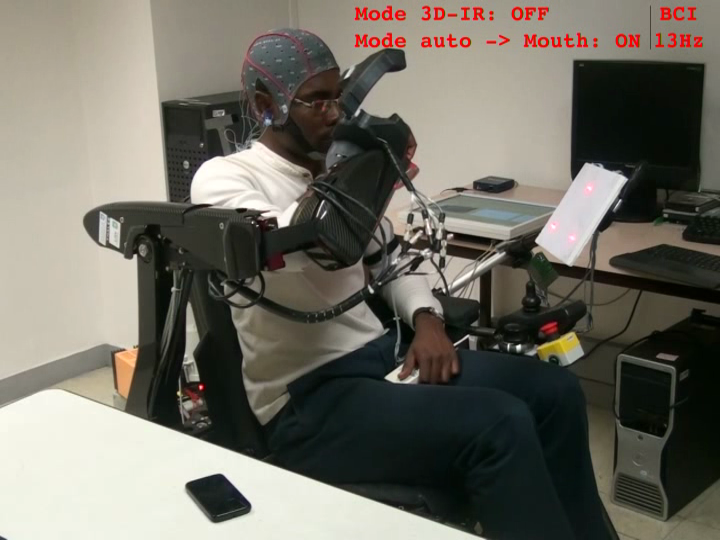
\includegraphics[width=0.45\textwidth]{Figures/esta04}
\label{fig:esta04}
}
\caption{Subject sitting on the ESTA wheelchair. His arm is supported by the exoskeleton, and the left hand is lying on the touchless interface. On his right-hand side is the SSVEP stimulation board. He is fitted with an EEG cap for brain signals recording. Next to the exoskeleton, an object is put on a table. (a) The subject is in resting position. He is gazing at the 17 Hz LED to trigger an automatic trajectory to the table. (b) Subject has reached the table and is using the touchless interface to reach and grab the glass (c) Glass in hand, the user gazing at the 13 Hz LED to activate the automatic trajectory to mouth. (d) The arm reaches the mouth while the touchless interface is deactivated.} 
\label{fig:esta-expe}
\end{figure} 
%\begin{figure}[!t]
%  \centering
%  %\pgfimage[interpolate=true,width=0.8\columnwidth]{Figures/online-esta.jpg}
%  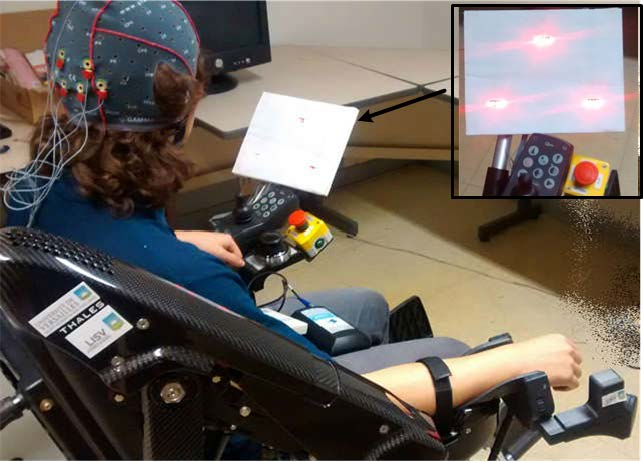
\includegraphics[width=0.8\columnwidth]{Figures/online-esta.jpg}
%  \caption{The ESTA arm exoskeleton with the proposed system: a 3D-touchless interface and the SSVEP-based BCI.}
%  \label{fig:online-esta-setup}
%\end{figure}


%%%%%%%%%%%%%%%%%%%%%%%%%%%%%%%%%%%%%%%%%%%%%%%%%%%%%%%%%%%%%%%%%%%%%%%%%%%%%%%%
\section{Conclusion}
\label{hBCI-conclusion}

In this chapter a new methodology for designing hybrid systems was proposed. It uses a brain interface and physical interface specifically design to fit the user's needs. 
The main goal of this hybrid system is to assist people with motor disabilities or muscular diseases, by proposing a system that adapts to their individual needs, and makes use of their residual abilities.
The BCI is integrated in the system as a secondary modality, which is used to trigger specific behaviour or predefined actions.

A first contribution is to propose an implementation of such a system using a 3D touchless interface and a SSVEP-based BCI.
This implementation gathers the two interfaces in a multimodal system which benefits from both the brain and motor signals.
The second contribution is to describe a novel algorithm for processing SSVEP-based EEG signals, with stable results, even when computed in an online setup.
This algorithm is compared to other existing solutions and an experimental assessment of its validity is conducted.

The full system is evaluated on a 3D  navigation task in virtual environment. 
The results demonstrate that the system is functional and could be used to assist people in various contexts.
The system is lastly used to control the ESTA arm exoskeleton: the system is functional and could be adapted for controlling other  assistive devices.

Although a good classification accuracy is achieved with the proposed method based on CCA and SVM, this work focuses more on BCI framework to improve the BCI usability and adaptability to the physical needs of subjects. The proposed framework answers the problem of variability in physical aptitude amongst patients and users of BCI.
Future work will be focused on the signal processing and machine learning methods that tackle variability in the brain response and in the experimental environment. 
%This continuous adaptation to the user's condition could help 
%speak of the aspect of maintaining both motor activity while lightening and/or fastening the task to be achieved with BCI.